\documentclass{article}
\usepackage{amsmath}
\usepackage{amsthm}
\usepackage{amssymb}
\usepackage{amsfonts}
\usepackage{mathtools}
\usepackage{listings}
\title{MATH 620: Homework 4}
\author{Fernando}
\date{\today}
\begin{document}
\maketitle
\section*{Problem 1}
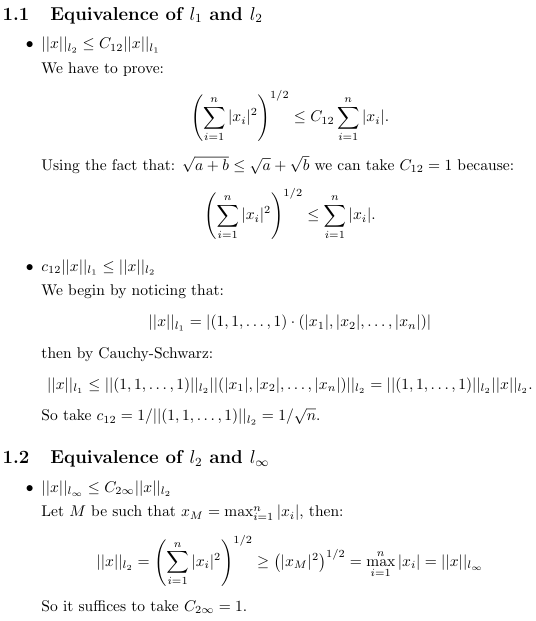
\includegraphics[width=0.99\textwidth]{prob1Part1hw4.png}

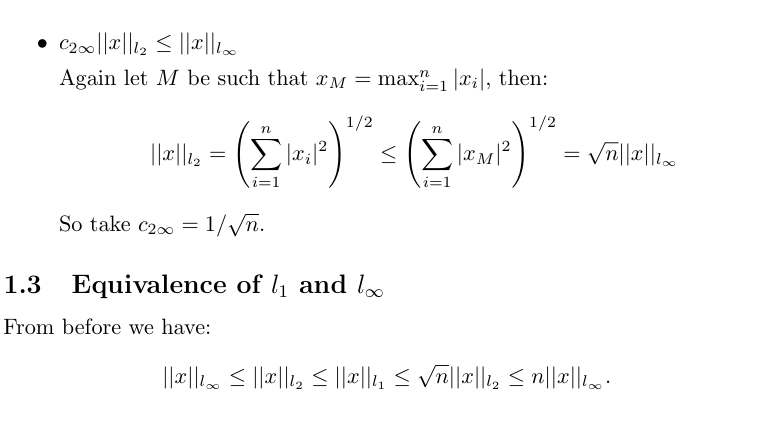
\includegraphics[width=0.95\textwidth]{prob1Part2hw4.png}
\section*{Problem 2}
\subsection*{Norm axioms}
\subsubsection*{$||\cdot||_1$}
All the axioms follow from the properties of the $\max$
\begin{itemize}
\item $\max_{x\in[0.1]}|au(x)|=|a|\max_{x\in[0.1]}|u(x)|$
\item $\max_{x\in[0.1]}|u(x)|=0 \implies \forall x \in [0,1] (|u(x)|\leq 0) \implies u\equiv0$
\item $\max_{x\in[0.1]}|u(x)+v(x)| \leq \max_{x\in[0.1]}|u(x)|+\max_{x\in[0.1]}|v(x)|$
\end{itemize}
The last statement is true because if we find $x_M$ that maximizes the sum $u+v$
then 
\begin{align*}
\max_{x\in[0.1]}|(u+v)(x)|= |(u+v)(x_M)|&\leq|u(x_M)|+|v(x_M)|\\
					&\leq\max_{x\in[0.1]}|u(x)|+\max_{x\in[0.1]}|v(x)|.
\end{align*}
\subsubsection*{$||\cdot||_2$}
Notice that $||u||_2=||u||_1+||u'||_1$. So all the norm requirements follow
from the fact that $||\cdot||_1$ is a norm and that the derivative is linear.
\subsubsection*{$||\cdot||_3$}
In these case the only property that is not immediate is the triangular
inequality. So let's proof that.

By Cauchy-Schwarz:
\[
	\int_0^1|u||v|\leq \left( \int_0^1|u|^2\right)^{1/2} 
	\left(\int_0^1|v|^2\right)^{1/2}
\]
Then:
\begin{align*}
	\int_0^1|u+v|^2&=\int_0^1|u|^2+\int_0^1|v|^2+2\int_0^1uv\\
		&\leq\int_0^1|u|^2+\int_0^1|v|^2+2\int_0^1|u||v|\\
		&\leq\int_0^1|u|^2+\int_0^1|v|^2+2\left(
		\int_0^1|u|^2\right)^{1/2}\left(\int_0^1|v|^2\right)^{1/2}\\
		&=\left(\left(\int_0^1|u|^2\right)^{1/2}+\left(\int_0^1|v|^2\right)^{1/2}\right)^2.
\end{align*}
Taking the square root we obtain the result.
\subsection*{Equivalence of norms}
No two norms are equivalent in this case. Notice that a consequence of the definition of
equivalence of norms is the following:

If $||\cdot||_a$ and $||\cdot||_b$ are equivalent then any sequence that is
convergent in $||\cdot||_a$ must also be convergent to the same limit point in
$||\cdot||_b$. This is because $x_n\to x$ in norm $||\cdot||_a$ means
$||x_n-x||_a\to 0$, and due to the equivalence of norms
\[
	||x_n-x||_b\leq c ||x_n-x||_a
\]
we have
\[
	||x_n-x||_b\to 0.
\]
\subsubsection*{$||\cdot||_1$ vs $||\cdot||_2$}
Since $||u||_2=||u||_1+||u'||_1$ it is clear that convergence in $||\cdot||_2$
implies convergence in $||\cdot||_1$ but the converse is not true.
Pick for example $x_n=x^n/n$. It is easy to see that $x_n\to 0$ in
$||\cdot||_1$ but because $\frac{d}{dx}(x^n/n)=x^{n-1}$ then $||x_n||_2=1$.
So $x_n\nrightarrow 0$ in $||\cdot||_2$. So these norms are not equivalent.
\subsubsection*{$||\cdot||_1$ vs $||\cdot||_3$}
Notice that:
\[
||\cdot||_3^2=\int_0^1|u|^2\leq \int_0^1 ||u||_1^2=||u||_1^2.
\]
So convergence in $||\cdot||_1$ implies convergence in $||\cdot||_3$. But the
converse is not true. Consider $x_n=x^n$. Clearly $||\cdot||_1=1$ but
$||x_n||_3=(1/(2n+1))^{1/2}$. So $x_n \to 0$ in $||\cdot||_3$ but
$x_n\nrightarrow 0$ in $||\cdot||_1$. So these norms are not equivalent.
\subsubsection*{$||\cdot||_2$ vs $||\cdot||_3$}
Convergence in $||\cdot||_2$ implies convergence in $||\cdot||_1$ which in turn
implies convergence in $||\cdot||_3$, but the converse is not true. Take the
same example as before. Again these norms are not equivalent.
\section*{Problem 3}
\section*{Problem 4}
\end{document}
